\include{header}
\usepackage{macros}

\author{
\Large
Homework 3: Building Your Neural Network! 
}


\begin{document}

\maketitle

This assignment is focusing on understanding the fundamental properties of neural networks and their training. 

\noindent\fbox{
    \parbox{\textwidth}{
        \textbf{Homework goals:} After completing this homework, you should be comfortable with: 
        \begin{itemize}
            \item thinking about neural networks 
            \item key implementation details of NNs, particularly in PyTorch, 
            \item explaining and deriving Backpropagation, 
            \item debugging your neural network in case it faces any failures. 
        \end{itemize}
    }
}

\vspace{0.5cm}


\additionalNotes


\clearpage

\section{Concepts, intuitions and big picture}

\begin{enumerate}
        \item Suppose you have built a neural network. You decide to initialize the weights and biases to be zero. Which of the following statements are True? (Check all that apply)\\
        \hspace{1cm}\checkedchoice{} Each neuron in the first hidden layer will perform the same computation. So even after multiple iterations of gradient descent each neuron will be computing the same thing as other neurons in the same layer.\\
        \hspace{1cm}\choice{} Each neuron in the first hidden layer will perform the same computation in the first iteration. But after one iteration of gradient descent they will learn to compute different things because we have ``broken symmetry''. \\ 
        \hspace{1cm}\choice{} Each neuron in the first hidden layer will compute the same thing, but neurons in different layers will compute different things, thus we have accomplished ``symmetry breaking'' as described in lecture. \\ 
        \hspace{1cm}\choice{} The first hidden layer's neurons will perform different computations from each other even in the first iteration; their parameters will thus keep evolving in their own way.\\
        \solution{}
    \item Vectorization allows you to compute forward propagation in an $L$-layer neural network without an explicit for-loop (or any other explicit iterative loop) over the layers $l=1, 2, \times, L$. True/False? \\ 
        \hspace{1cm}\checkedchoice{} True \\ 
        \hspace{1cm}\choice{} False\\
        \solution{}
    \item  The {\tt tanh} activation usually works better than sigmoid activation function for hidden units because the mean of its output is closer to zero, and so it centers the data better for the next layer.  True/False? \\ 
        \hspace{1cm}\checkedchoice{} True \\ 
        \hspace{1cm}\choice{} False \\ 
        \solution{}

    \item Which of the following techniques does NOT prevent a model from overfitting? \\ 
        \hspace{1cm}\choice{} Data augmentation
        \hspace{1cm}\choice{} Dropout
        \hspace{1cm}\choice{} Early stopping
        \hspace{1cm}\checkedchoice{} None of the above\\
    \solution{}
    \item Why should dropout be applied during training? Why should dropout NOT be applied during evaluation?\\
    \solution{
        The number of parameters and scale of NN allows for massive degrees of overfitting. Dropout is used to prevents NN to be overreliant and "Memorizing" certain
        patterns in the data. Instead by dropping out certain aspects of network prevents overreliance and forces the "understanding" of general patterns. This Is
        only practical during the training phase as that is when these parameters are being chosen. If dropout were applied during evaluation it would create
        inconsistencies in the results of the data as well as not truly testing the model but simply a subset or similar model.
    }
    \item Explain why initializing the parameters of a neural net with a constant is a bad idea. \\
    \solution{
        Similar to the previously mentioned problem of setting all to 0 by putting all parameters to the same constant will result in the same operation
        being performed on all parameters and will make each layers parameters identical to another.
    }
    \item You design a fully connected neural network architecture where all activations are sigmoids. You initialize the weights with large positive numbers. Is this a good idea? Explain your answer.\\
    \solution{
        No this will create something similar to constant problem. Since the sigmoid function is capped between 0-1 large numbers will generally be mapped to 1 essentially
        setting it as a the constant 1.
    }

    \item Explain what is the importance of ``residual connections''. \\
    \solution{
        Residual connections is a way to reapply weight of information earlier inside of the neural network later on this decreases the negative impact that
        vanishing gradients have on the model. allowing for a more accurate impact on the model.
    }
        
        \item What is cached (``memoized'') in the implementation of forward propagation and backward propagation?\\
        \hspace{1cm}\checkedchoice{}  Variables computed during forward propagation are cached and passed on to the corresponding backward propagation step to compute derivatives.\\
        \hspace{1cm}\choice{} Caching is used to keep track of the hyperparameters that we are searching over, to speed up computation.\\
        \hspace{1cm}\choice{} Caching is used to pass variables computed during backward propagation to the corresponding forward propagation step. It contains useful values for forward propagation to compute activations.\\
        \solution{}
    \item Which of the following statements is true?\\
        \hspace{1cm}\checkedchoice{} The deeper layers of a neural network are typically computing more complex features of the input than the earlier layers. \\ 
        \hspace{1cm}\choice{} The earlier layers of a neural network are typically computing more complex features of the input than the deeper layers. \\
        \solution{}
\end{enumerate}

   






\section{Revisiting Jacobians}
Recall that Jacobians are generalizations of multi-variate derivatives and are extremely useful in denoting the gradient computations in computation graph and Backpropagation.
A potentially confusing aspect of using Jacobains is their dimensions and so, here we're going focus on understanding Jacobian dimensions. 


\noindent
\paragraph{Recap:}Let's first recap the formal definition of Jacobian. 
Suppose $\mathbf{f}: \reals^n \rightarrow \reals^m $ is a function takes a point $\mathbf{x} \in \reals^n$  as input and produces the vector $\mathbf{f(x)} \in \reals^m$ as output. 
Then the Jacobian matrix of  $\mathbf{f}$ is defined to be an $m \times n$ matrix, denoted by $\mathbf{J}_\mathbf{f}(\mathbf{x})$, whose $(i, j)$th entry is $\mathbf{J}_{ij} = \frac{\partial f_i}{\partial x_j}$, or: 

$$
\mathbf J = \begin{bmatrix}
  \dfrac{\partial \mathbf{f}}{\partial x_1} & \cdots & \dfrac{\partial \mathbf{f}}{\partial x_n}
\end{bmatrix}
= \begin{bmatrix}
  \nabla^{\top} f_1 \\  
  \vdots \\
  \nabla^{\top} f_m   
\end{bmatrix}
= \begin{bmatrix}
    \dfrac{\partial f_1}{\partial x_1} & \cdots & \dfrac{\partial f_1}{\partial x_n}\\
    \vdots                             & \ddots & \vdots\\
    \dfrac{\partial f_m}{\partial x_1} & \cdots & \dfrac{\partial f_m}{\partial x_n}
\end{bmatrix}
$$

% where <math>\nabla^{\mathrm T} f_i </math> is the transpose (row vector) of the [[gradient]] of the <math>i</math>-th component.

\noindent
\paragraph{Examples:}The shape of a Jacobian is an important notion to note. A Jacobian can be a vector, a matrix, or a tensor of arbitrary ranks. Consider the following special cases: 
\begin{itemize}
    \item If $f$ is a scalar and $\textbf{w}$ is a $d \times 1$ column vector, the Jacobian of $f$ with respect to \textbf{w} is a row vector with $1 \times d$ dimensions.
    \item If $\textbf{y}$ is a $n \times 1$ column vector and $\textbf{z}$ is a $d \times 1$ column vector, the Jacobian of $\mathbf{z}$ with respect to $y$, or $\textbf{J}_\textbf{z}(\textbf{y})$ is a $d \times n$ matrix.  
    \item Suppose $\textbf{A} \in \reals^{m\times n}$ and  $\mathbf{B} \in \reals^{l\times p \times q}$. Then  the Jacobian $\textbf{J}_\textbf{A}({\textbf{B}})$  is a tensor of shape $(m \times n) \times (l \times p \times q)$. 
    More broadly, the shape of the Jacobian is determined as (shape of the output)$\times$(shape of the input).
\end{itemize}



\noindent \paragraph{Problem setup:}Suppose we have:
\begin{itemize}
    \item $X$, an $n \times d$ matrix, $x_i \in \reals^{d\times 1}$ correspond to the rows of $X = [x_1, \hdots, x_n]^\top$
    \item $Y$, a $n \times k$ matrix
    \item $W$, a $k \times d$ matrix and $w$, a $d \times 1$ vector
    % \item $Z$, an $n \times k$ matrix
\end{itemize}

For the following items, compute 
{\underline{(1) the shape of each Jacobian, and (2) an expression for each Jacobian}}:
\begin{enumerate}
    \item $f(w) = c$ (constant) \\ 
        \solution{    
        \[
            \frac{d}{dw}\left( f(w)\right) = 0
        \]}
    \item $f(w) = \|w\|^2$ (squared L2-norm) \\ 
        \solution{   
            \[
            \frac{d}{dw}\left( f(w)\right) = 
            2w
            \]
        }
    \item $f(w) = w^\top x_i$ (vector dot product)\\
        \solution{  
            \[
            \frac{d}{dw}\left( f(w)\right) = 
            x_i
            \]
        }
    \item $f(w) = Xw$ (matrix-vector product) \\ 
        \solution{
            \[
            \frac{d}{dw} = X
            \]
            %\[
            %\frac{d}{dx}_1 = 
            %\begin{bmatrix}
            %    w_{0,0} & w_{1,0} & w_{2,0} \cdots & w_{n,0} \\
            %    w_{0,0} & w_{1,0} & w_{2,0} \cdots & w_{n,0} \\
            %\end{bmatrix}
            %\]
        }
    \item $f(w) = w$ (vector identity function)\\ 
        \solution{\[
        \begin{bmatrix}
            1 \\ 1 \\ 1 \\ \vdots \\ 1
        \end{bmatrix}
        \]}
    \item $f(w) = w^2$ (element-wise power)\\
        \solution{$2w$}
    \item \extracredit{} $f(W) =  X W^\top$ (matrix multiplication)\\
        \solution{\[
            \frac{dX}{dW} =  X
        \]}
\end{enumerate}

\clearpage


\section{Activations Per Layer, Keeps Linearity Away!}
\label{sec: activation}
Based on the content we saw at the class lectures, answer the following: 
\begin{enumerate}
    \item Why are activation functions used in neural networks? 
    \solution{
        Because not all functions are linearly separable and therefore require a different activatioon function to be properly modeled by a neural network.
        in other words it increases the expressive power of the neural network. :)
    }
    \item Write down the formula for three common action functions (sigmoid, ReLU, Tanh) and their derivatives (assume scalar input/output). 
    Plot these activation functions and their derivatives on $(-\infty, +\infty)$. 
    \solution{
        Sigmoid functions
        \[
            f(x)=\frac{1}{1-e^{-x}}
        \]
        \[
            f'(x)=\frac{e^{-x}}{\left( 1-e^{-x}\right)^2}
        \]
        ReLU Function
        \[
            f(x)=\max\left( 0,x\right)
        \]
        \[
            f'(x)=
            \begin{cases} 
                1 & : x > 0 \\
                0 & : x < 0
            \end{cases}
        \]
        Tanh Function
        \[
            f(x)=\tanh\left( x\right)
        \]
        \[
            f'(x)=1-\tanh^2\left(x\right)
        \]
    }
    \item What is the ``vanishing gradient'' problem? (respond in no more than 3 sentences) Which activation functions are subject to this issue and why? (respond in no more than 3 sentences). \\
    \solution{
        Vanishing gradients is a problem where as you move backwards through a network the gradients tend to shrink and therefore slow down gradient descent and the
        program all together. It is overall a problem with functions that saturate including $\tanh$ and Sigmoid.
    }
    \item Why zero-centered activation functions impact the results of Backprop? \\
    \solution{
        Zero centered functions are generallt problematic because it damages the ability for a function to move in opposite directions allowing for both sides allows
        for a wide range of mtions that a vector can have on its output
    }
    \item Remember the Softmax function $\sigma(\textbf{z})$ and how it extends sigmoid to multiple dimensions? Let's compute the derivative of Softmax for each dimension. Prove that: 
        $$
        \frac{ d \sigma(\mathbf{z})_i }{ d z_j } = \sigma(\mathbf{z})_i (\delta_{ij} - \sigma(\mathbf{z})_j)
        $$
        where $\delta_{ij}$ is the Kronecker delta function.\footnote{
        \url{https://en.wikipedia.org/wiki/Kronecker_delta}
        }
        \solution{
            Firstly we will solve assuming i==j
            \[
            \frac{d}{dx} \sigma\left( \mathbf{z} \right) = \frac{d}{dx} \frac{e^{z_i}}{\sum_{k=1}^{n} e^{z_k}}
            \]
            \[
            e^{z_i} \left( \sum_{k=1}^{n} e^{z_k} \right)^{-1} - e^{z_i} e^{z_i} \left( \sum_{k=1}^{n} e^{z_k} \right)^{-2}
            \]
            \[
            e^{z_i} \left( \sum_{k=1}^{n} e^{z_k} \right)^{-1} \left( 1 - e^{z_i} \left( \sum_{k=1}^{n} e^{z_k} \right)^{-1} \right)
            \]
            \[
            \sigma_i\left(\mathbf{z} \right) \left( 1 - \sigma_j\left(\mathbf{z} \right) \right)
            \]
            Then secondly we assume i!=j
            \[
            \frac{d}{dx} \sigma\left( \mathbf{z} \right) = \frac{d}{dx} \frac{e^{z_i}}{\sum_{k=1}^{n} e^{z_k}}
            \]
            \[
                \frac{d}{dx} e^{z_i} \left( \sum_{k=1}^{n}\right)^{-1} - e^{z_i}
            \]
            \[
                - e^{z_i} \left( \sum_{k=1}^{n}\right)^{-2}e^{z_j}
            \]
            \[
                - \sigma_i\left( \mathbf{z}\right) \sigma_j\left( \mathbf{z}\right)
            \]
            \[
                \sigma_i\left(\mathbf{z}\right) \left( 0 - \sigma_j \mathbf{z}\right)
            \]
            This shows that we fulfill the cases for the krunker delta and can insert it for both 1 and 0 in the respective functions
        }
    \item Use the above point to prove that the Jacobian of the Softmax function is the following: 
    $$
    \mathbf{J}_{\sigma}(\mathbf{z}) = \text{diag}(\sigma(\mathbf{z})) - \sigma(\mathbf{z}) \sigma(\mathbf{z})^\top
    $$
    where $\text{diag}(.)$ turns a vector into a diagonal matrix. 
    Also, note that 
    $
    \mathbf{J}_{\sigma}(\mathbf{z}) \in \reals^{K \times K}. 
    $.\\
    \solution{
        Firstly lets consider a diagonal where i == j
        \[
            \sigma_i\left(e^{\z_i}\right) - \sigma_i\left(e^{z_i}\right)\sigma_j\left(e^{z_i}\right)
        \]
        \[
            \sigma_i\left(e^{\z_i}\right) \left(1 - \sigma_j\left(e^{z_i}\right) \right)
        \]
        Which is our expected result
        \[
            0 - \sigma_i\left(e^{z_i}\right)\sigma_j\left(e^{z_i}\right)
        \]
        \[
            \sigma_i\left(e^{\z_i}\right) \left(0 - \sigma_j\left(e^{z_i}\right) \right)
        \]
        Therefore the formula holds.
    }
\end{enumerate}





\section{Simulating XOR}
\begin{enumerate}
    \item Can a single-layer network simulate (represent) an XOR function on $\mathbf{x} = [x_1, x_2]$? 
    $$
    y = \text{XOR}(\mathbf{x}) = 
    \begin{cases}
        1, & \text{if } \mathbf{x} = (0, 1) \text{ or } \mathbf{x} = (1, 0) \\ 
        0, & \text{if } \mathbf{x} = (1, 1) \text{ or } \mathbf{x} = (0, 0).
    \end{cases}
    $$
    Explain your reasoning using the following single-layer network definition:  $\hat{y} = \text{ReLU}(W \cdot \mathbf{x} +b)$
    \solution{
        First lets assume it does hold in which case we must have solutions to the following equations
        \[
            W_0x_0 + w_1x_1 + b =0 
        \]
        \[
            W_0x_0 +b = 1
        \]
        \[
            W_1x_1 +b = 1
        \]
        \[
            b = 0
        \]
        \[
            W_0x_0 = 1 - b
        \]
        \[
            W_1x_1 = 1 - b
        \]
        Plugging that into the first equation we generate
        \[
            1 - b + 1 - b =0
        \]
        \[
         2 = 2b
        \]
        \[
            b = 1
        \]
        This a contradiction with $b = 0$
    }
    \item Repeat (1) with a two-layer network: 
    \begin{align*}
        \mathbf{h} = \text{ReLU}(W_1 \cdot \mathbf{x} +\mathbf{b}_1)\\ 
        \hat{y} = W_2 \cdot \mathbf{h} + b_2
    \end{align*}
    Note that this model has an additional layer compared to the earlier question: an input layer $\textbf{x}\in \reals^2$, a
    hidden layer $\textbf{h}$ with ReLU activation functions that are applied component-wise, and
    a linear output layer, resulting in scalar prediction $\hat{y}$. Provide a set of weights $W_1$ and $W_2$ and biases $\textbf{b}_1$ and $b_2$ such that this model can accurately model the XOR problem.
    \\
    \solution{
        An answer for this would be
        \[
            W_1 = \begin{bmatrix}
                1 & 1 \\
                1 & -1
            \end{bmatrix}
            b_1 = \begin{bmatrix}
                0 \\ 0
            \end{bmatrix}
            W_2 = \begin{bmatrix}
                1 & -1
            \end{bmatrix}
            b_2 = 0
        \]
        Doing the respective calculations we get the following
        \[
            \text{ReLU}(W \cdot \mathbf{\begin{bmatrix}
                0 \\ 0
            \end{bmatrix}} +b) = 0
        \]
        \[
            \text{ReLU}(W \cdot \mathbf{\begin{bmatrix}
                0 \\ 1
            \end{bmatrix}} +b) = 1
        \]
        \[
            \text{ReLU}(W \cdot \mathbf{\begin{bmatrix}
                1 \\ 0
            \end{bmatrix}} +b) = 1
        \]
        \[
            \text{ReLU}(W \cdot \mathbf{\begin{bmatrix}
                1 \\ 1
            \end{bmatrix}} +b) = 0
        \]
    }
    \item Consider the same network as above (with ReLU activations for the hidden layer), with an arbitrary differentiable loss function $\ell : \set{0, 1} × \set{0, 1} \rightarrow \reals$ which takes as input $\hat{y}$ and $y$, our prediction and ground truth labels, respectively. 
    Suppose all weights and biases are initialized to zero. 
    Show that a model trained using standard gradient descent will not learn the XOR function given this initialization.\\
    \solution{
        Gradient Descent will fail here as setting everything to 0 is essentially the 0 function and every index will be 0 so all indexes will have following calculations
        \[f(x) = 0\]
        \[f'(x) = 0\]
        and wont be trained
    }
  
\end{enumerate}

\clearpage

\begin{wraptable}[7]{r}{7.4cm}
\vspace{-2cm}
 \begin{framed}
 \footnotesize
A computation graph, so elegantly designed\\
With nodes and edges, so easily combined\\
It starts with inputs, a simple array \\
 And ends with outputs, in a computationally fair way \\\\ 
Each node performs, an operation with care\\
And passes its results, to those waiting to share\\
The edges connect, each node with its peers\\
And flow of information, they smoothly steer\\\\
It's used to calculate, complex models so grand\\
And trains neural networks, with ease at hand\\
Backpropagation, it enables with grace\\
Making deep learning, a beautiful race

\hspace{4cm}--ChatGPT Feb 3 2023 
\end{framed}
\end{wraptable}
\section{Neural Nets and Backpropagation}
Draw the computation graph for $f(x, y, z) = \ln x + \exp(y) \cdot z$. Each node in the graph should correspond to only one simple operation (addition, multiplication, exponentiation, etc.). Then we will follow the forward and backward propagation described in class to estimate the value of $f$ and partial derivatives $\frac{\partial f}{\partial x}, \frac{\partial f}{\partial y}, \frac{\partial f}{\partial z}$ at $[x, y, z] = [1, 3, 2]$. For each step, show you work.  \\ \\ \\
    

    
    \begin{enumerate}
            \item Draw the computation graph for $f(x, y, z) = \ln x + \exp(y) \cdot z$. The graph should have three input nodes for $x, y, z$ and one output node $f$. Label each intermediate node $h_i$. \\
            
            \solution{
                \begin{figure}[h]
                    \centering
                    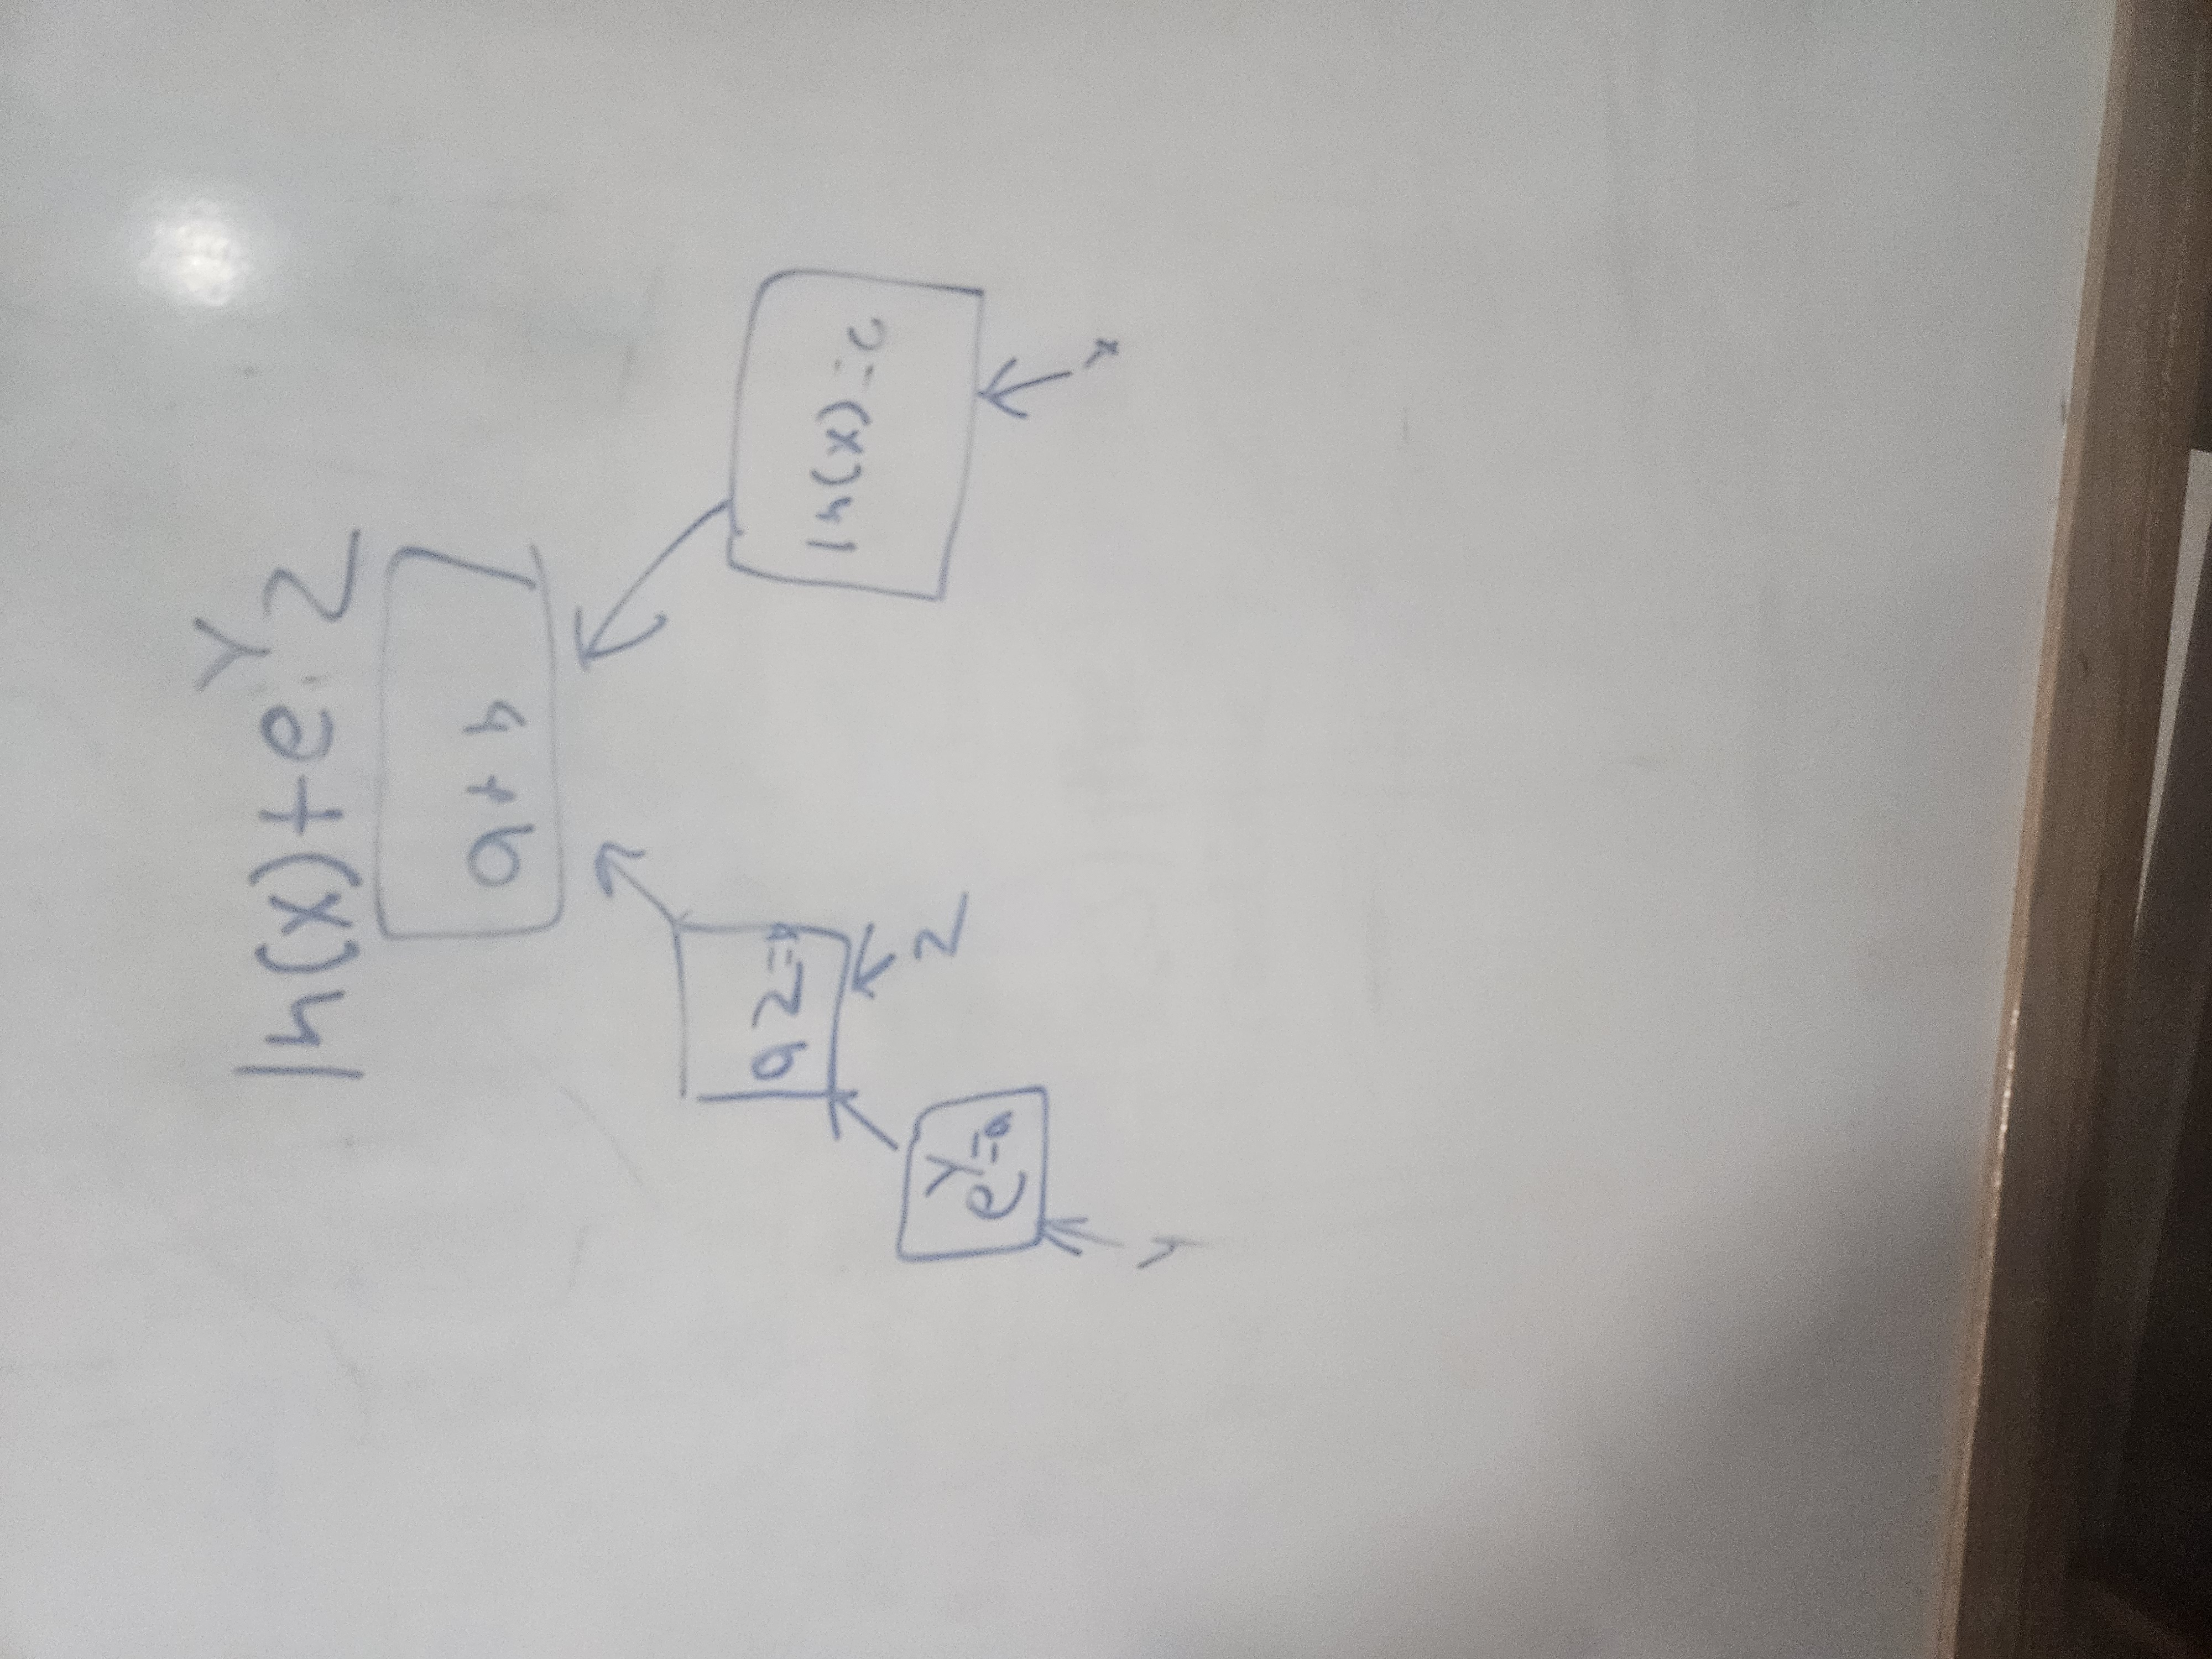
\includegraphics[width=0.5\textwidth]{figures/Diagram.jpg}
                    \caption{Computation graph for $f(x, y, z)$}
                \label{fig:example}
                \end{figure}
            }
            \item Run the forward propagation and evaluate $f$ and $h_i$ ($i=1, 2, \dots$) at $[x, y, z] = [1, 3, 2]$.\\
            \solution{
                \[
                h_1 = \ln x = \ln 1 = 0
                \]
                \[
                h_2 = e^y = e^3
                \]
                \[
                h_3 = h_2 \cdot z = e^3 \cdot 2 = 2e^3
                \]
                \[
                f = h_1 + h_3 = 0 + 2e^3 = 2e^3
                \]
            }
            \item Run the backward propagation and give partial derivatives for each intermediate operation, i.e., $\frac{\partial h_i}{\partial x}$, $\frac{\partial h_j}{\partial h_i}$, and $\frac{\partial f}{\partial h_i}$. Evaluate the partial derivatives at $[x, y, z] = [1, 3, 2]$.\\
            \solution{
                \[
                \frac{\partial h_1}{\partial x} = \frac{1}{x}
                \]
                \[
                \frac{\partial h_2}{\partial y} = e^y
                \]
                \[
                \frac{\partial h_3}{\partial h_2} = z
                \]
                \[
                \frac{\partial h_3}{\partial z} = h_2
                \]
                \[
                \frac{\partial f}{\partial h_1} = 1
                \]
            }
            \item Aggregate the results in (c) and evaluate the partial derivatives $\frac{\partial f}{\partial x}$, $\frac{\partial f}{\partial y}$, $\frac{\partial f}{\partial z}$ using the chain rule. Show your work.\\
            \solution{
                \[
                \quad \frac{\partial h_1}{\partial x}(1)  = 1
                \]
                \[
                \frac{\partial h_2}{\partial y}(3)= e^3
                \]
                \[
                \frac{\partial h_3}{\partial h_2(2)}= 2
                \]
                \[
                \frac{\partial h_3}{\partial z}(e^3)  = e^3
                \]
                \[
                \frac{\partial f}{\partial h_3} = 1
                \]
            }
    \end{enumerate}



\clearpage

\section{Programming}
In this programming homework, we will
\begin{itemize}
    \item implement MLP-based classifiers for the sentiment classification task of homework 1.
\end{itemize}
\noindent \paragraph{Skeleton Code and Structure:}
The code base for this homework can be found at MyClasses Files under the \texttt{hw3} directory. Your task is to fill in the missing parts in the skeleton code, following the requirements, guidance, and tips provided in this pdf and the comments in the corresponding .py files.
The code base has the following structure:
\begin{itemize}
    \item \texttt{mlp.py} reuse the sentiment classifier on movie reviews you implemented in homework 1, with additional requirements to implement MLP-based classifier architectures and forward pass .
    \item \texttt{main.py} provides the entry point to run your implementations \texttt{mlp.py}
    \item \texttt{hw3.md} provides instructions on how to setup the environment and run each part of the homework in \texttt{main.py}
\end{itemize}
\noindent \todo{} ---
Your tasks include
1) generate plots and/or write short answers based on the results of running the code; 2) fill in the blanks in the skeleton to complete the code. We will explicitly mark these plotting, written answer, and filling-in-the-blank tasks as \todo{} in the following descriptions, as well as a \textcolor{blue}{\texttt{\textbf{\#~TODO}}} at the corresponding blank in the code. \\
\noindent \todo{} (Copy from your HW1). We are reusing most of the \texttt{model.py} from homework 1 as the starting point for the \texttt{mlp.py} - you will see in the skeleton that they look very similar. Moreover, in order to make the skeleton complete, for all the \textcolor{blue}{\texttt{\textbf{\#~TODO (Copy from your HW1)}}}, please fill in the blank below them by copying and pasting the corresponding implementations you wrote for homework 1 (i.e. the corresponding \textcolor{blue}{\texttt{\textbf{\#~TODO}}} in homework 1.)
\noindent \paragraph{Submission:} Your submission should contain two parts: 1) plots and short answers under the corresponding questions below; and 2) your completion of the skeleton code base, in a \texttt{.zip} file
\subsection{MLP-based Sentiment Classifier}
In both homework 1 \& 2, our implementation of the \texttt{SentimentClassifer} is essentially a single-layer feedforward neural network that maps input features directly to 2-dimensional output logits. In this part of the programming homework, we will expand the architecture of our classifier to multi-layer perceptron (MLP). 
\subsubsection{Reuse Your HW1 Implementation}
\todo{} (Copy from your HW1): for all the \textcolor{blue}{\texttt{\textbf{\#~TODO (Copy from your HW1)}}} in \texttt{mlp.py}, please fill in the blank below them by copying and pasting the corresponding implementations you wrote for homework 1 (i.e. the corresponding \textcolor{blue}{\texttt{\textbf{\#~TODO}}} in the \texttt{model.py} in homework 1).
\subsubsection{Build MLPs}
\label{subsubsec: build mlps}
Remember from the lecture that MLP is a multi-layer feedforward network with perceptrons as its nodes. A perceptron consists of non-linear activation of the affine (linear) transformation of inputs.
\\\\
\noindent \todo{}: Complete the \texttt{\_\_init\_\_} and \texttt{forward} function of the \texttt{SentimentClassifier} class in \texttt{mlp.py} to build MLP classifiers that supports custom specification of architecture (i.e. number and dimension of hidden layers)\\
\noindent \textbf{Hint}: check the comments in the code for specific requirements about input, output, and implementation. Also, check out the document of \href{https://pytorch.org/docs/stable/generated/torch.nn.ModuleList.html}{nn.ModuleList} about how to define and implement forward pass of MLPs as a stack of layers.
\subsubsection{Train and Evaluate MLPs}
We provide in \texttt{main.py} several MLP configurations and corresponding recipes for training them.\\\\
\noindent\todo{} Once you finished \autoref{subsubsec: build mlps}, you can run \texttt{load\_data\_mlp} and \texttt{explore\_mlp\_structures} to train and evaluate these MLPs and paste two sets of plots here:
\begin{itemize}
    \item 4 plots of train \& dev loss for each MLP configuration
    \item 2 plots of dev losses and accuracies across MLP configurations
\end{itemize}
and describe in 2-3 sentences your findings.\\
\noindent \textbf{Hint}: what are the trends of train \& dev loss and are they consistent across different configurations? Is deeper models always better? Why?\\
\noindent {\color{red}{your plots and answer:}}\\
% uncomment the following blocks to include your plots
\begin{figure}[h] 
    \centering
    \subfloat[No Hidden Layer]{
        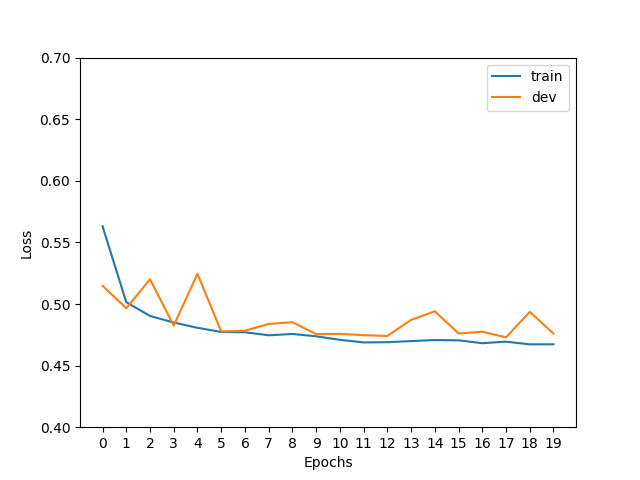
\includegraphics[width=0.23\textwidth]{mlp_structure_None_loss.png}
        }
    \hfill
    \subfloat[1 Hidden Layer]{
        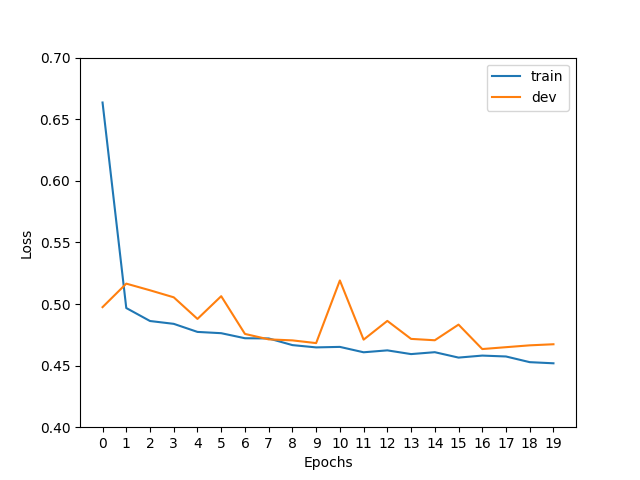
\includegraphics[width=0.23\textwidth]{mlp_structure_512_loss.png}
        }
    \hfill
    \subfloat[2 Hidden Layers]{
        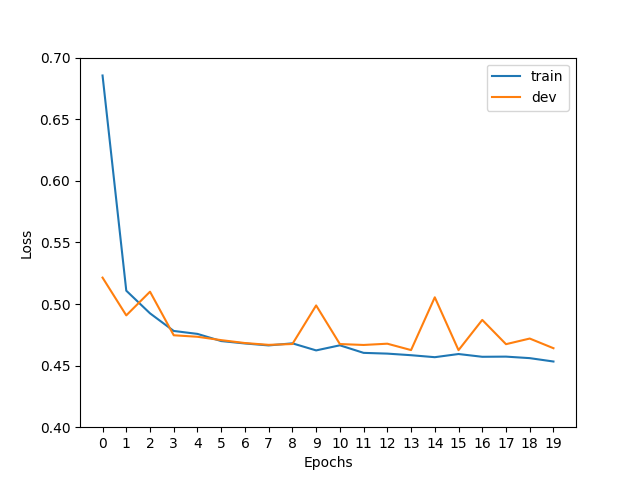
\includegraphics[width=0.23\textwidth]{mlp_structure_512 -> 512_loss.png}
        }
    \hfill
    \subfloat[3 Hidden Layers]{
        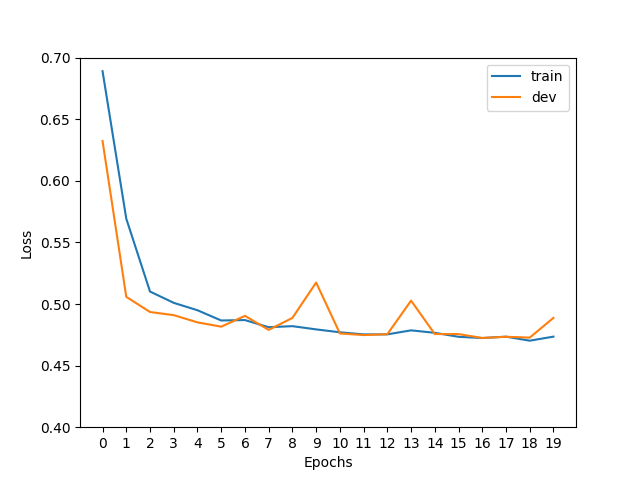
\includegraphics[width=0.23\textwidth]{mlp_structure_512 -> 512 -> 512_loss.png}
        }
    \caption{loss of different MLP architectures}
\end{figure}
\begin{figure}[h] 
    \centering
    \subfloat[dev loss of different MLP architectures]{
        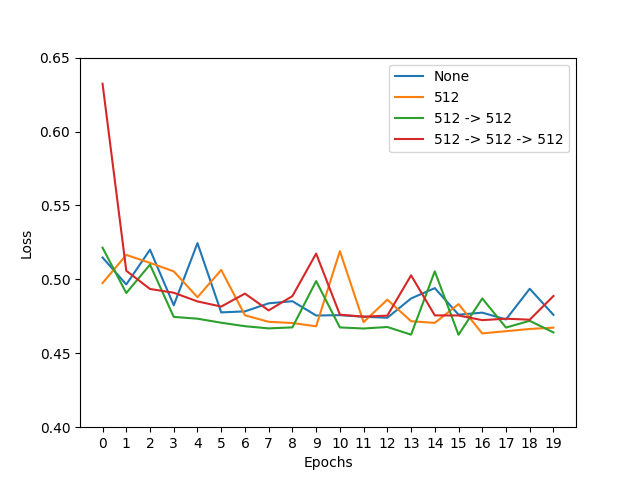
\includegraphics[width=0.45\textwidth]{all_mlp_structures_loss.png}
        }
    \hfill
    \subfloat[dev acc of different MLP architectures]{
        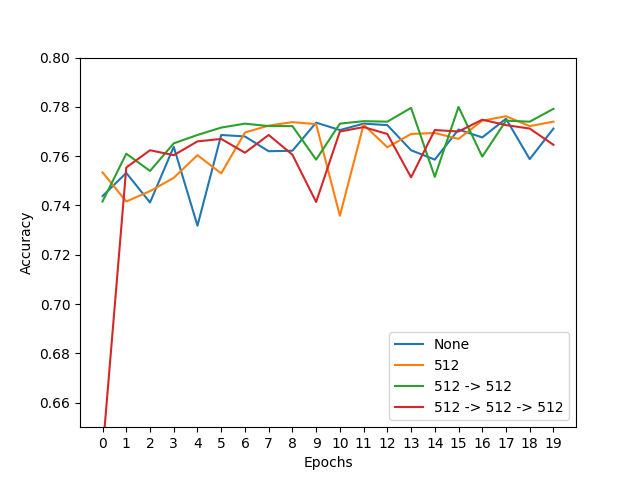
\includegraphics[width=0.45\textwidth]{all_mlp_structures_acc.png}
        }
    \caption{loss and acc of different MLP architectures}
\end{figure}    
\solution{
    We can see off the models below a quite surprising result that smaller models seem to perform better having generally higher accuracy and lower loss. 
    One potential reason for this is Vanishing and exploding gradients where increased layers result in reduced ability to train models. We can also see that
    the initial accuacies of the smaller models perform better potentially due to ability to train smaller models quicker given less parameters.
}
\subsubsection{Embrace Non-linearity: The Activation Functions}
Remember we have learned why adding non-linearity is useful in neural nets and gotten familiar with several non-linear activation functions both in the class and \autoref{sec: activation}. Now it is time to try them out in our MLPs! \\
\textbf{Note: for the following TODO and the TODO in \autoref{subsubsec: lr}, we fix the MLP structure to be with a single 512-dimension hidden layer, as specified in the code. You only need to run experiments on this architecture}.\\\\
\noindent\todo{}: Read and complete the missing lines of the two following functions:
\begin{itemize}
    \item \texttt{\_\_init\_\_} function of the \texttt{SentimentClassifier} class: define different activation functions given the input \texttt{activation} type.\\
    \textbf{Hint}: we have provided you with a demonstration of defining the Sigmoid activation, you can search for the other \texttt{nn.<activation>} in PyTorch documentation.\\
    \item \texttt{explore\_mlp\_activations} in \texttt{main.py}: iterate over the activation options, define the corresponding training configurations, train and evaluate the model, and visualize the results. Note: you only need to generate the plots of dev loss and dev acc across different configurations, by calling \texttt{visualize\_configs}, you \textbf{do not} need to plot the train-dev loss curves for each configuration (i.e. no need to call \texttt{visualize\_epochs}). We provide you with a few choices of common activation functions, but feel free to try out the others.\\
    \textbf{Hint}: You can refer to \texttt{explore\_mlp\_structure} as a demonstration of how to define training configurations with fixed hyper-parameters \& iterate over hyper-parameters/design choices of interests (e.g. hidden dimensions, choice of activation), and plot the evaluation results across configurations. 
\end{itemize}
Once you complete the above functions, run \texttt{explore\_mlp\_activations} and paste the two generated plots here. Describe in 2-3 sentences your findings.\\
\noindent {\color{red}{your plots and answer:}}\\
% uncomment the following blocks to include your plots
\begin{figure}[h] 
    \centering
    \subfloat[dev loss of different activations]{
        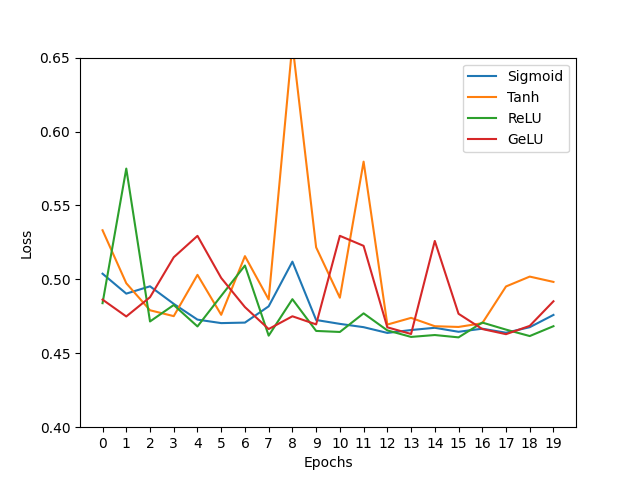
\includegraphics[width=0.45\textwidth]{all_mlp_activations_loss.png}
        }
    \hfill
    \subfloat[dev acc of different MLP architectures]{
        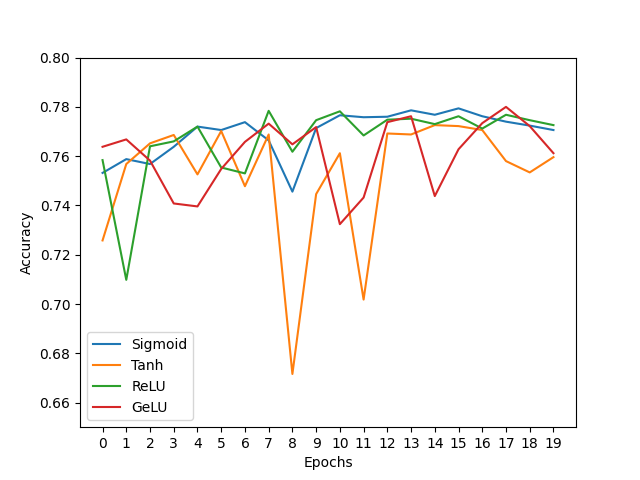
\includegraphics[width=0.45\textwidth]{all_mlp_activations_acc.png}
        }
    \caption{loss and acc of different activations}
\end{figure}\\
\solution{
    Based on results we see Sigmoid and ReLu are the best activation functions on average with Sigmoid generally performing better. We also can see that
    That these functions tend to be the more stable of the four.
}
\subsubsection{Hyper-parameter Tuning: Learning Rate}
\label{subsubsec: lr}
The training process mostly involves learning model parameters, which are automatically performed by gradient-based methods. However, certain parameters are ``unlearnable" through gradient optimization while playing a crucial role in affecting model performance, for example, learning rate and batch size. We typically refer to these parameters as \textit{Hyper-parameters}.

We will now take the first step to tune these hyper-parameters by exploring the choices of one of the most important one - learning rate, on our MLP. (There are lots of tutorials on how to tune the learning rate manually or automatically in practice, for example \href{https://www.kaggle.com/code/residentmario/tuning-your-learning-rate}{this note} can serve as a starting point.)\\\\
\noindent\todo{}: Read and complete the missing lines in \texttt{explore\_mlp\_learning\_rates} in \texttt{main.py} to iterate over different learning rate values, define the training configurations, train and evaluate the model, and visualize the results. Note: same as above, you only need to generate the plots of dev loss and dev acc across different configurations, by calling \texttt{visualize\_configs}, you \textbf{do not} need to plot the train-dev loss curves for each configuration (i.e. no need to call \texttt{visualize\_epochs}). We provide you with the default learning rate we set to start with, and we encourage you to add more learning rate values to explore and include in your final plots curves of \textbf{at least 4 different representative learning rates.}\\
\noindent\textbf{Hint}: again, you can checkout \texttt{explore\_mlp\_structure} as a demonstration for how to perform hyper-parameter search.\\
Once you complete the above functions, run \texttt{explore\_mlp\_learning\_rates} and paste the two generated plots here. Describe in 2-3 sentences your findings.\\
\noindent {\color{red}{your plots and answer:}}\\
% uncomment the following blocks to include your plots
\begin{figure}[h] 
    \centering
    \subfloat[dev loss of different learning rates]{
        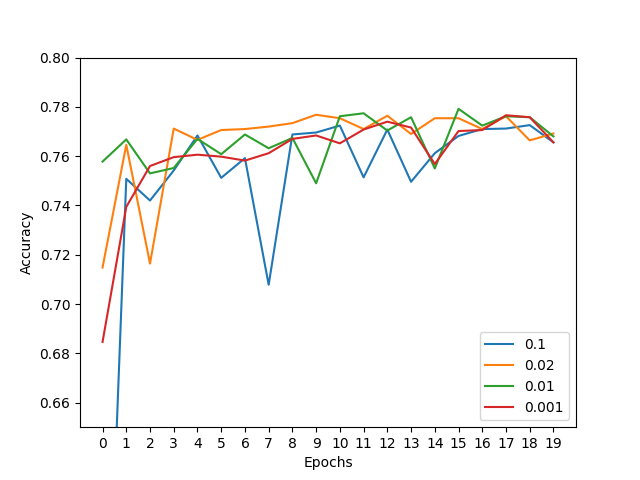
\includegraphics[width=0.45\textwidth]{all_mlp_lrs_acc.png}
        }
    \hfill
    \subfloat[dev acc of different MLP architectures]{
        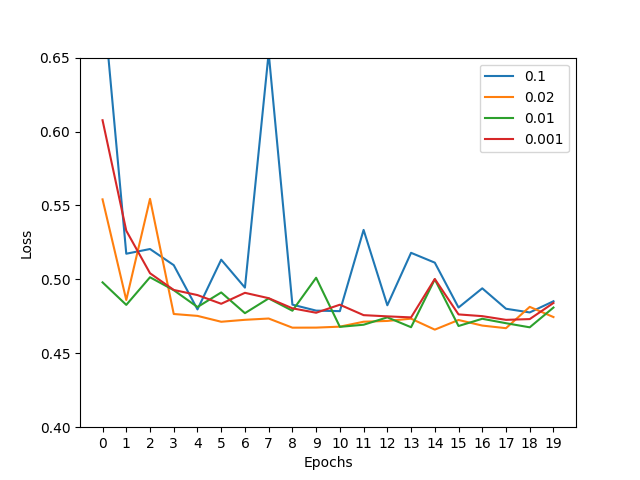
\includegraphics[width=0.45\textwidth]{all_mlp_lrs_loss.png}
        }
    \caption{loss and acc of different learning rates}
\end{figure}\\
\bibliographystyle{apalike}
\bibliography{ref}
\noindent\solution{
    In the long run given a high number of epochs there isnt much difference between learning rates which makes sense as they should all be converging to the same value.
    However in the short term we see high learning rates results in more spratic changes but in general faster convergence while lower learning rates are the opposite.
}
\end{document}
\bibliographystyle{apalike}
\bibliography{ref}
\end{document}